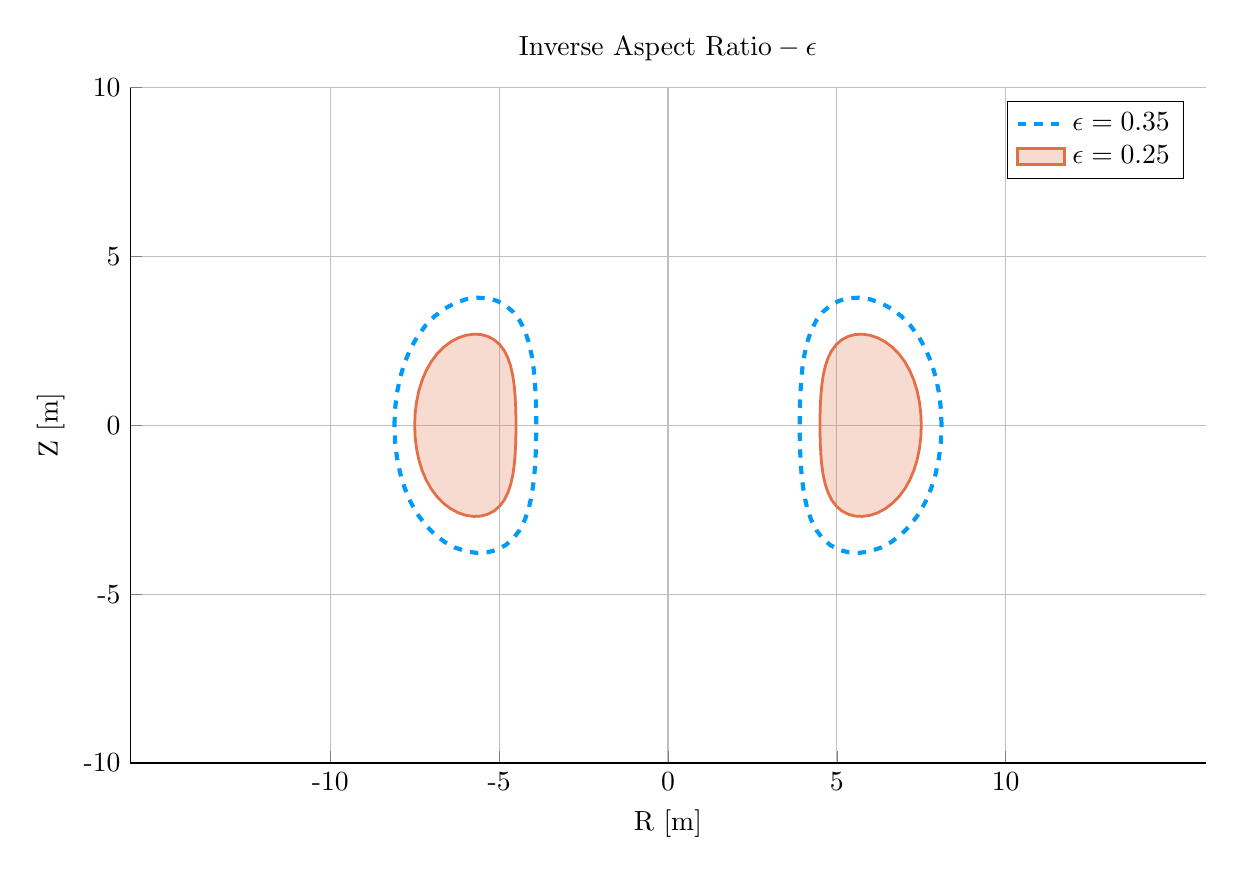
\begin{tikzpicture}[]
\begin{axis}[height = {101.6mm}, axis equal = {true}, ylabel = {Z [m]}, title = {$\textnormal{Inverse Aspect Ratio} - \epsilon$}, xmin = {-10}, xmax = {10}, ymax = {10}, xlabel = {R [m]}, {unbounded coords=jump, scaled x ticks = false, xticklabel style={rotate = 0}, xmajorgrids = true, xtick = {-10.0,-5.0,0.0,5.0,10.0}, xticklabels = {-10,-5,0,5,10}, xtick align = inside, axis lines* = left, scaled y ticks = false, yticklabel style={rotate = 0}, ymajorgrids = true, ytick = {-10.0,-5.0,0.0,5.0,10.0}, yticklabels = {-10,-5,0,5,10}, ytick align = inside, axis lines* = left,     xshift = 0.0mm,
    yshift = 0.0mm,
    axis background/.style={fill={rgb,1:red,1.00000000;green,1.00000000;blue,1.00000000}}
}, ymin = {-10}, width = {152.4mm}]\addplot+ [color = {rgb,1:red,0.00000000;green,0.60560316;blue,0.97868012},
draw opacity=1.0,
line width=1.5,
dashed,mark = none,
mark size = 2.0,
mark options = {
    color = {rgb,1:red,0.00000000;green,0.00000000;blue,0.00000000}, draw opacity = 1.0,
    fill = {rgb,1:red,0.00000000;green,0.60560316;blue,0.97868012}, fill opacity = 1.0,
    line width = 1,
    rotate = 0,
    solid
}]coordinates {
(8.1, 0.0)
(8.081204069972497, 0.48337567116743263)
(8.024684777757766, 0.9588143271779377)
(7.930141280572084, 1.4185092784440338)
(7.797367695668915, 1.854912346574885)
(7.626640572703316, 2.260857805256796)
(7.419158721180681, 2.6296800412811785)
(7.177452352825953, 2.9553230037291525)
(6.905679431512412, 3.232439644160208)
(6.609741255084048, 3.456479714999771)
(6.297174663233395, 3.623764484478577)
(5.976811190071814, 3.7315471413066206)
(5.658229090447864, 3.7780578972385994)
(5.351057127458824, 3.7625330469479685)
(5.06421429716898, 3.685227508047293)
(4.805183334632925, 3.547410635348094)
(4.579415603765742, 3.3513453780899396)
(4.389950548568067, 3.100251122376493)
(4.237306076467235, 2.7982508289446923)
(4.119660690046763, 2.45030333426344)
(4.033308834588962, 2.0621219265758737)
(3.9733333500050683, 1.6400805338643698)
(3.9344084806536994, 1.1911090641292867)
(3.911628010194501, 0.7225796164911881)
(3.9012485454184915, 0.24218543152709598)
(3.9012485454184915, -0.2421854315270951)
(3.911628010194501, -0.7225796164911872)
(3.9344084806536994, -1.1911090641292859)
(3.9733333500050687, -1.640080533864369)
(4.033308834588962, -2.0621219265758732)
(4.119660690046763, -2.450303334263439)
(4.237306076467235, -2.7982508289446915)
(4.389950548568066, -3.1002511223764917)
(4.579415603765742, -3.3513453780899396)
(4.8051833346329245, -3.5474106353480934)
(5.064214297168979, -3.685227508047293)
(5.351057127458825, -3.7625330469479685)
(5.658229090447862, -3.7780578972385994)
(5.976811190071814, -3.731547141306621)
(6.297174663233394, -3.6237644844785772)
(6.609741255084048, -3.456479714999771)
(6.90567943151241, -3.232439644160209)
(7.177452352825952, -2.955323003729153)
(7.419158721180681, -2.629680041281178)
(7.626640572703316, -2.260857805256797)
(7.797367695668915, -1.854912346574885)
(7.930141280572083, -1.4185092784440358)
(8.024684777757766, -0.9588143271779382)
(8.081204069972497, -0.483375671167435)
(8.1, -9.258329801553988e-16)
};
\addlegendentry{$\epsilon = 0.35$}
\addplot+ [color = {rgb,1:red,0.00000000;green,0.60560316;blue,0.97868012},
draw opacity=1.0,
line width=1.5,
dashed,mark = none,
mark size = 2.0,
mark options = {
    color = {rgb,1:red,0.00000000;green,0.00000000;blue,0.00000000}, draw opacity = 1.0,
    fill = {rgb,1:red,0.00000000;green,0.60560316;blue,0.97868012}, fill opacity = 1.0,
    line width = 1,
    rotate = 0,
    solid
},forget plot]coordinates {
(-8.1, 0.0)
(-8.081204069972497, 0.48337567116743263)
(-8.024684777757766, 0.9588143271779377)
(-7.930141280572084, 1.4185092784440338)
(-7.797367695668915, 1.854912346574885)
(-7.626640572703316, 2.260857805256796)
(-7.419158721180681, 2.6296800412811785)
(-7.177452352825953, 2.9553230037291525)
(-6.905679431512412, 3.232439644160208)
(-6.609741255084048, 3.456479714999771)
(-6.297174663233395, 3.623764484478577)
(-5.976811190071814, 3.7315471413066206)
(-5.658229090447864, 3.7780578972385994)
(-5.351057127458824, 3.7625330469479685)
(-5.06421429716898, 3.685227508047293)
(-4.805183334632925, 3.547410635348094)
(-4.579415603765742, 3.3513453780899396)
(-4.389950548568067, 3.100251122376493)
(-4.237306076467235, 2.7982508289446923)
(-4.119660690046763, 2.45030333426344)
(-4.033308834588962, 2.0621219265758737)
(-3.9733333500050683, 1.6400805338643698)
(-3.9344084806536994, 1.1911090641292867)
(-3.911628010194501, 0.7225796164911881)
(-3.9012485454184915, 0.24218543152709598)
(-3.9012485454184915, -0.2421854315270951)
(-3.911628010194501, -0.7225796164911872)
(-3.9344084806536994, -1.1911090641292859)
(-3.9733333500050687, -1.640080533864369)
(-4.033308834588962, -2.0621219265758732)
(-4.119660690046763, -2.450303334263439)
(-4.237306076467235, -2.7982508289446915)
(-4.389950548568066, -3.1002511223764917)
(-4.579415603765742, -3.3513453780899396)
(-4.8051833346329245, -3.5474106353480934)
(-5.064214297168979, -3.685227508047293)
(-5.351057127458825, -3.7625330469479685)
(-5.658229090447862, -3.7780578972385994)
(-5.976811190071814, -3.731547141306621)
(-6.297174663233394, -3.6237644844785772)
(-6.609741255084048, -3.456479714999771)
(-6.90567943151241, -3.232439644160209)
(-7.177452352825952, -2.955323003729153)
(-7.419158721180681, -2.629680041281178)
(-7.626640572703316, -2.260857805256797)
(-7.797367695668915, -1.854912346574885)
(-7.930141280572083, -1.4185092784440358)
(-8.024684777757766, -0.9588143271779382)
(-8.081204069972497, -0.483375671167435)
(-8.1, -9.258329801553988e-16)
};
\addplot+ [color = {rgb,1:red,0.88887350;green,0.43564919;blue,0.27812294},
draw opacity=1.0,
line width=1,
solid,mark = none,
mark size = 2.0,
mark options = {
    color = {rgb,1:red,0.00000000;green,0.00000000;blue,0.00000000}, draw opacity = 1.0,
    fill = {rgb,1:red,0.88887350;green,0.43564919;blue,0.27812294}, fill opacity = 1.0,
    line width = 1,
    rotate = 0,
    solid
},fill = {rgb,1:red,0.88887350;green,0.43564919;blue,0.27812294}, fill opacity=0.25,area legend]coordinates {
(7.5, 0.0)
(7.486574335694641, 0.34526833654816624)
(7.446203412684119, 0.6848673765556699)
(7.378672343265774, 1.0132209131743102)
(7.283834068334939, 1.3249373904106323)
(7.161886123359512, 1.6148984323262832)
(7.013684800843344, 1.8783428866294134)
(6.841037394875681, 2.1109450026636805)
(6.646913879651723, 2.3088854601144346)
(6.435529467917177, 2.468914082142694)
(6.212267616595282, 2.588403203198984)
(5.98343656433701, 2.6653908152190153)
(5.755877921748474, 2.6986127837418574)
(5.536469376756303, 2.687523604962835)
(5.331581640834985, 2.632305362890924)
(5.146559524737804, 2.533864739534353)
(4.985296859832673, 2.3938181272071004)
(4.84996467754862, 2.214465087411781)
(4.74093291176231, 1.998750592103352)
(4.6569004928905455, 1.7502166673310287)
(4.595220596134973, 1.4729442332684815)
(4.552380964289334, 1.1714860956174071)
(4.524577486181213, 0.8507921886637764)
(4.508305721567501, 0.5161282974937058)
(4.500891818156065, 0.17298959394792573)
(4.500891818156065, -0.1729895939479251)
(4.508305721567501, -0.5161282974937051)
(4.524577486181213, -0.8507921886637757)
(4.552380964289334, -1.1714860956174067)
(4.595220596134973, -1.472944233268481)
(4.656900492890545, -1.7502166673310282)
(4.74093291176231, -1.9987505921033515)
(4.849964677548619, -2.21446508741178)
(4.985296859832673, -2.3938181272071004)
(5.146559524737803, -2.5338647395343528)
(5.331581640834985, -2.632305362890924)
(5.536469376756303, -2.687523604962835)
(5.755877921748473, -2.6986127837418574)
(5.98343656433701, -2.6653908152190153)
(6.212267616595281, -2.5884032031989843)
(6.435529467917177, -2.468914082142694)
(6.646913879651722, -2.3088854601144355)
(6.841037394875681, -2.110945002663681)
(7.013684800843344, -1.878342886629413)
(7.161886123359511, -1.6148984323262838)
(7.283834068334939, -1.3249373904106323)
(7.378672343265773, -1.0132209131743115)
(7.446203412684119, -0.6848673765556703)
(7.486574335694641, -0.3452683365481679)
(7.5, -6.613092715395707e-16)
};
\addlegendentry{$\epsilon = 0.25$}
\addplot+ [color = {rgb,1:red,0.88887350;green,0.43564919;blue,0.27812294},
draw opacity=1.0,
line width=1,
solid,mark = none,
mark size = 2.0,
mark options = {
    color = {rgb,1:red,0.00000000;green,0.00000000;blue,0.00000000}, draw opacity = 1.0,
    fill = {rgb,1:red,0.88887350;green,0.43564919;blue,0.27812294}, fill opacity = 1.0,
    line width = 1,
    rotate = 0,
    solid
},fill = {rgb,1:red,0.88887350;green,0.43564919;blue,0.27812294}, fill opacity=0.25,forget plot]coordinates {
(-7.5, 0.0)
(-7.486574335694641, 0.34526833654816624)
(-7.446203412684119, 0.6848673765556699)
(-7.378672343265774, 1.0132209131743102)
(-7.283834068334939, 1.3249373904106323)
(-7.161886123359512, 1.6148984323262832)
(-7.013684800843344, 1.8783428866294134)
(-6.841037394875681, 2.1109450026636805)
(-6.646913879651723, 2.3088854601144346)
(-6.435529467917177, 2.468914082142694)
(-6.212267616595282, 2.588403203198984)
(-5.98343656433701, 2.6653908152190153)
(-5.755877921748474, 2.6986127837418574)
(-5.536469376756303, 2.687523604962835)
(-5.331581640834985, 2.632305362890924)
(-5.146559524737804, 2.533864739534353)
(-4.985296859832673, 2.3938181272071004)
(-4.84996467754862, 2.214465087411781)
(-4.74093291176231, 1.998750592103352)
(-4.6569004928905455, 1.7502166673310287)
(-4.595220596134973, 1.4729442332684815)
(-4.552380964289334, 1.1714860956174071)
(-4.524577486181213, 0.8507921886637764)
(-4.508305721567501, 0.5161282974937058)
(-4.500891818156065, 0.17298959394792573)
(-4.500891818156065, -0.1729895939479251)
(-4.508305721567501, -0.5161282974937051)
(-4.524577486181213, -0.8507921886637757)
(-4.552380964289334, -1.1714860956174067)
(-4.595220596134973, -1.472944233268481)
(-4.656900492890545, -1.7502166673310282)
(-4.74093291176231, -1.9987505921033515)
(-4.849964677548619, -2.21446508741178)
(-4.985296859832673, -2.3938181272071004)
(-5.146559524737803, -2.5338647395343528)
(-5.331581640834985, -2.632305362890924)
(-5.536469376756303, -2.687523604962835)
(-5.755877921748473, -2.6986127837418574)
(-5.98343656433701, -2.6653908152190153)
(-6.212267616595281, -2.5884032031989843)
(-6.435529467917177, -2.468914082142694)
(-6.646913879651722, -2.3088854601144355)
(-6.841037394875681, -2.110945002663681)
(-7.013684800843344, -1.878342886629413)
(-7.161886123359511, -1.6148984323262838)
(-7.283834068334939, -1.3249373904106323)
(-7.378672343265773, -1.0132209131743115)
(-7.446203412684119, -0.6848673765556703)
(-7.486574335694641, -0.3452683365481679)
(-7.5, -6.613092715395707e-16)
};
\end{axis}

\end{tikzpicture}
